\documentclass{article}
\author{Harrison Coons, Steve Doolan, Sam Throne}
\title{Delayed Differential Equations for Cloud Computing}
\date{\today}
\usepackage{enumitem}
\usepackage{algorithmic}
\usepackage{graphicx}
\usepackage{caption}
\usepackage{subcaption}
\usepackage{amsmath}
\usepackage{enumerate}
\usepackage{float}
\begin{document}
\maketitle

\section{Delayed Differential Equation Models}
\subsection{Introduction}
Load balancing is a common computer networking method used by cloud processes including could computing. Load balancing seeks to distribute tasks to minimize task completion time and take advantage of available resources. Doing so requires communication between cores and is affected by delays. This model looks at three core computing cluster as seen in Figure \ref{diagram}. 
\begin{figure}[ht]
\begin{center} 
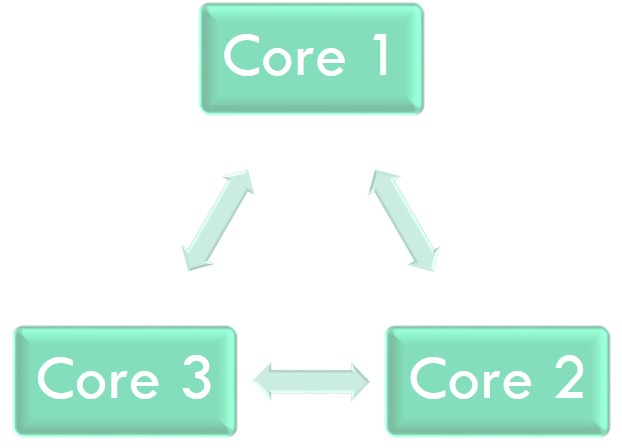
\includegraphics[width=0.4\linewidth]{model.jpg}
\caption{Layout of the Computing Cluster}\label{diagram}
\end{center}
\end{figure}
\\All of the cores in the cluster are capable of transferring packets from their respective queues to the other cores. Each core has both the ability to process packets and send them off, and therefor must decide how it should allocate its processing power. Each core was assigned different values for power and maximum queue size , as well as distinct input function. The cluster as a whole had defined delay values for communication and transfer, a shared  history, and a minimum queue percentage. 



Two delayed differential equation models were created. The first set of DDEs were used to model the size of the queue of each of the processors. The second set of DDEs were used to model the `pipe' between any set of two processors. These pipes act as holding queues that delay information transfer between processors and will be discussed in more detail in a subsequent section.

\subsection{Definitions}

The following nomenclature describes the model. 

\begin{itemize}
\item $q_i(t)$ - amount of data in queue $i$ at time $t$
\item $I_i$ - inflow of data into queue $i$, this is set and may be time-dependent
\item $T_{mn}$ - rate of data transfer from queue $m$ to queue $n$
\item $P_i$ - processing power of queue $i$
\item $k_T$ - cost of data transfer (e.g. $k_T = 0.1$ means that transferring data would require 10 percent of the processing power required to process the data)
\item $k_r$ - the remainder coefficient for distributing data to other processors. 
\item $d$ - the damping coefficient further explained in section something
\item $\tau$ - time delay
\item $s_i$ - maximum size of queue $i$
\end{itemize}

In addition, the following indices were used.

\begin{itemize}
\item $i$ - indexes the queue
\item $h$ - indexes the pipe between queues
\end{itemize}



\subsection{Queue Management}\label{Queue Managment}
All packets coming in to the cluster were sent to different queues as related to the individual input functions. Once in the queue they waited in line to be processed. Each queue could be divided in to three sections. The first section, is reserved for the next packets up for processing, and everything in it is locked from being transfered to other cores. This section represents a space defined by the equation:
\[size = \left(Queue Size\right) \cdot Minimum Queue Percentage \quad . \]
The middle section is made up of packets waiting to be processed that are able to be transfered to other cores. This section is made up of all packets not in the first section. Finally, the third section is available space, and consists of what the space not used by the first or second sections. 
\\ The cluster handles the load balancing using the following algorithm: 
%\begin{multline}\nonumber
\[T_{mn}=d\frac{q_m \left(t- \tau \right)-k_rS_m}{\sum^{3}_{j=1}w_j}w_m\]
\[w_j =\frac{\left(s_j -q_j \left(t-\tau\right)\right)P_j}{\sum^{3}_{k=1, k\neq j}\left(s_k-q_k\left(t-\tau\right)\right)P_k-\left(s_j-q_j\left(t\right)\right)P_j}\]
%\end{multline}
\noindent
The second equation sets up the proportional stiffness of each queue as a factor of the space remaining, processing power, and transfer delay.  Once established, the first equation then redistributes the packets in the second section of all of the queues. Because of real world delays for communication and packet transfer, the redistribution is further limited by the damping coefficient to prevent cores from shipping packets they no longer have. 



Once shipped, the packets transfer to the destination queue through a pipe equation which simulates the transfer delay. This equation is presented below:

\[
\frac{dq_i}{dt} = I_i + \sum_{h=1,h\ne i}^{3} T_{hi} - \sum_{h=1,h\ne i}^{3} T_{ih} - \left( P_i - k_T \sum_{h=1,h\ne i}^{3} T_{ih} \right).
\]

\noindent
The first term refers to the specified in-flow function, set by the user. This can be a time-dependent function. The second and third terms describe the transfers to and from pipes, respectively as referenced above. The final term represents the processing of information by the processor. The second term within the parentheses decreases processing power, $P_i$, based on the amount of information being transferred from the processor. 


\subsection{Pipe Size}

The derivative of the size of the `pipe' between two processors using a basic conservation approach was modeled with the sum of the amount going into the pipe and the amount leaving. A time delay was added to the in-flow term to account for the delay of information transfer. 

\[
\frac{dq_h}{dt} = \sum_{i=1}^{3} T_{ih}(t-\tau) - \sum_{i=1}^{3} T_{hi}(t)
\]

\noindent
The first term is the in-flow to the pipe, while the second term refers to the out-flow. The pipes were modeled as connecting two specific processors. Out of convenience, the summation ranges were written as $i=1$ to $3$. Please note that only two of the transfer amounts values will be non-zero for this range of indices.


\subsection{Time Delays in Model}\label{time delay}
To better model the real world system, a time delay was added to the model in two places, the first is in the communication between the cores where they tell each other how much information they each have, and the second delay is the transfer delay, which delays the receipt of previously transfered packets. To model the communications delay, in the computation where packet transfer is decided for an individual core, the callouts for the current time queue sizes are replaced by the callouts for queue sizes at a time of $t-\tau$ where $\tau=.5$ in the system time, with the exception of the core where the data transfer rates are being calculated from. The result of this delay was largely a slightly noticeable increase in the sinusoidal response of the system, as it would often cause one stack to become filled more than others, which would then fill excessively and require a dump to the other processors.For the transferal delay, the standard outflow rates are computed and subtracted from their respective computers, but that same rate is not added at a given time, instead the time rate from $t-\tau_2$ where $tau_2=1$ is used as the inflow to the systems computers. Since our model does not store data on where packets of data go once they leave the individual cores, a series of secondary differential equations were used to model this intermediate 'pipeline' where the data is flowing between two cores. This pipelines' rate of flow is what the cores receive as the inflow at a given time $t$ from the delay. This delay in transfer works to accentuate the delay in the communications and causes additional buildup-and-dump in packets which creates a sinusoidal time delay. 

To model this as a differential equation, the derivative of the size of the`pipe' between two processors is the transfer into the core. That is, we add the amount going into the pipe and subtract the amount leaving.

\[
\frac{dq_h}{dt} = \sum_{i=1}^{3} T_{ih}(t-\tau) - \sum_{i=1}^{3} T_{hi}(t)
\]

\noindent
The first term is the in-flow to the pipe, while the second term refers to the out-flow. We modeled the pipes as connecting two specific processors. Out of convenience, the summation ranges were written as $i=1$ to $3$. Please note that only two of the transfer amounts values will be non-zero for this range of indices.


\section{Model Results}

The results of the model are shown in the following plots of queue size that exhibit specific characteristics of the model. These characteristics are evident by comparing all of the created plots to a base plot. The base plot is shown below. 

\begin{figure}[H]
                \centering
                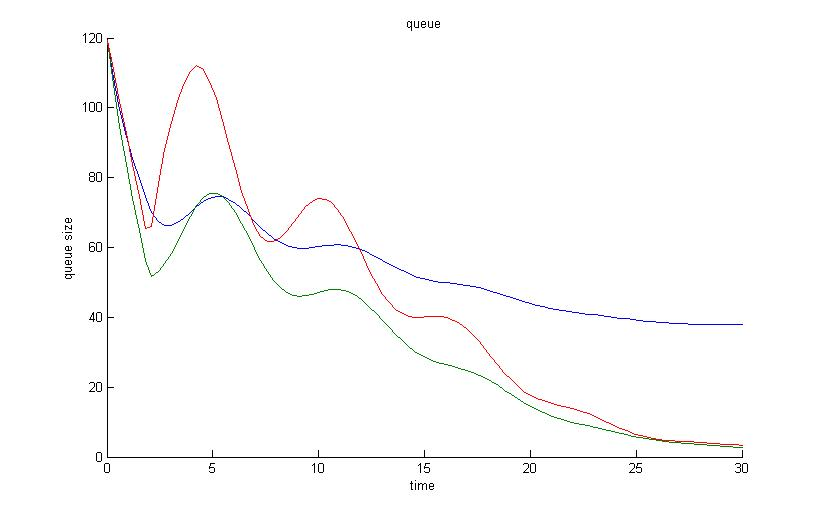
\includegraphics[width=.9\linewidth]{Normal}
                \caption{The base plot of the model.}
\end{figure}

\noindent
This model uses 
\begin{center}
\begin{tabular}{c|ccc}
                & \multicolumn{3}{c}{Value} \\
Parameter & Blue & Red & Green \\
\hline
$I$ & 50 & 0 & 0\\
$P$ & 10 & 20 & 30 \\
$s$ & 400 & 400 & 400 \\
history & 120 & 120 & 120 \\
\end{tabular}
\end{center}

\noindent
and

\begin{center}
\begin{tabular}{c|c}
Parameter & Value \\
\hline
$k_r$ & 0.01 \\
$d$ & 0.7 \\
$k_T$ & 0.05 \\
\end{tabular}
\end{center}

\noindent
as the specified parameters. These values are then changed to create show significant characteristics of the model. 

\subsection{Decision Making Delay}

As discussed in the queue management section,  a time delay was used in our DDE to create the decision making delay. The effect of this delay is shown in the figure below. 

\begin{figure}[H]
                \centering
                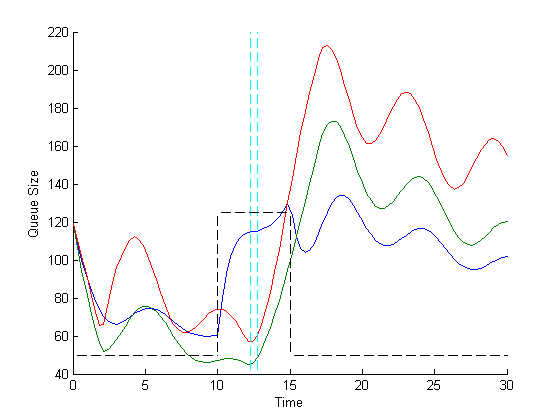
\includegraphics[width=0.8\linewidth]{Decision_making_delay}
                \caption{Queue size of the three processors with a Heaviside function input.}
\end{figure}

\noindent
Each solid line in the figure corresponds to a processor, while the black dashed line shows the input to the system. The difference between the cyan dashed lines indicate the duration of the decision making delay. The blue processor is the only processor that receives the input. This input is 

\[
I_{blue} = \left\{
\begin{array}{ll}
125 & : 10 \le t \le 15 \\
50 & : \mbox{else} \\
\end{array} \right.
\]


\noindent
When the input increases from 50 to 125 at $t=10$, the queue size of the blue processor immediately begins to increase. It maintains this high slope for the duration of a decision making time delay because the decision to send and receive information is based on the queue size before the dramatic input increase. After the duration of the decision making delay has passed the slope of the blue processor decreases because it begins transferring data. The slope does not become negative because the processor is still receiving the large input. 

The derivative of the queue of the blue processor approaches zero around $t=12$. At this point, the processor model indicates that it has a much higher queue than the other processors. As a result, it transfers as much information as possible. So much so that it is able to either process or transmit all of the input, as indicated by the zero slope. The point where the red and green processors begin to receive more information than they can process is indicated by the first cyan line. The blue processor continues to transfer out the same amount of information until after a decision making delay, indicated by the second dashed cyan line. After this time delay, the blue core transfers out less information because the queues of the red and green cores have increased. In other words, the first cyan line indicates the minimum value of the red and green queues. The queues begin to increase after the first cyan line. The second cyan line shows the last point where the blue core has a zero slope. After this point, the slope begins to increase because of the increase in the red and green queue sizes directly after the first cyan line. 

\subsection{Packet Transfer Delay}

We use a time delay in our DDE to create the packet transfer delay. The effect of this delay is shown in the figure below. This figure uses the same parameters as the original figure, however the third queue and the pipe between the second and third queues are shown. 

\begin{figure}[H]
                \centering
                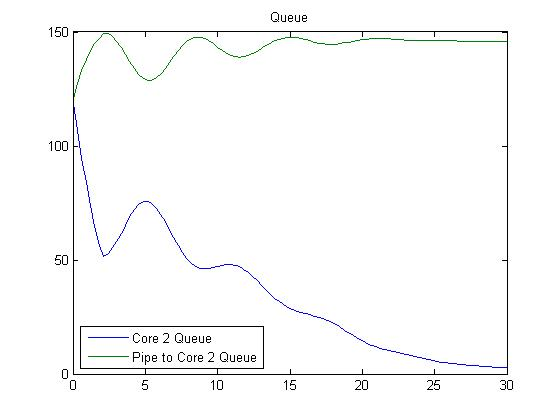
\includegraphics[width=0.8\linewidth]{Send_Receive_Delay}
                \caption{Queue 2 and Pipe 2 to 3 size.}
\end{figure}

\noindent
As discussed previously, the packet transfer delay was accounted for by delaying the transfer between packets exiting a queue and entering a pipe. Thus, a delay is expected from when packets are transferred out of queue three and into pipe 2-3. 

The first dashed cyan line is approximately the point where the number of packets entering the third queue equals the number exiting. After this point, the third queue will be sending more packets than it is receiving. These packets will enter the pipe between queues two and three after one time delay. This is represented by the second dashed cyan line, which is one time delay after the first. At this point the pipe begins to receive the packets that were sent from queue two one time delay earlier.  



\subsection{Variations in History and Forcing Input}

As the input function is one of the few factors of the model that can directly effect the number of tasks a computer has to do, one of the first things chosen to vary was the input to the first processor. In the default model shown in section \ref{default} uses a constant input value of 50 tasks/second with no variation over time. For the altered input function, a sin function following:

\begin{equation} 
input=25+25\cdot sin(t\cdot4)
\end{equation}

a graph using this input function is shown below given the same time scale as the default graph.

\begin{figure}[h]
\label{Sin input}
\centering
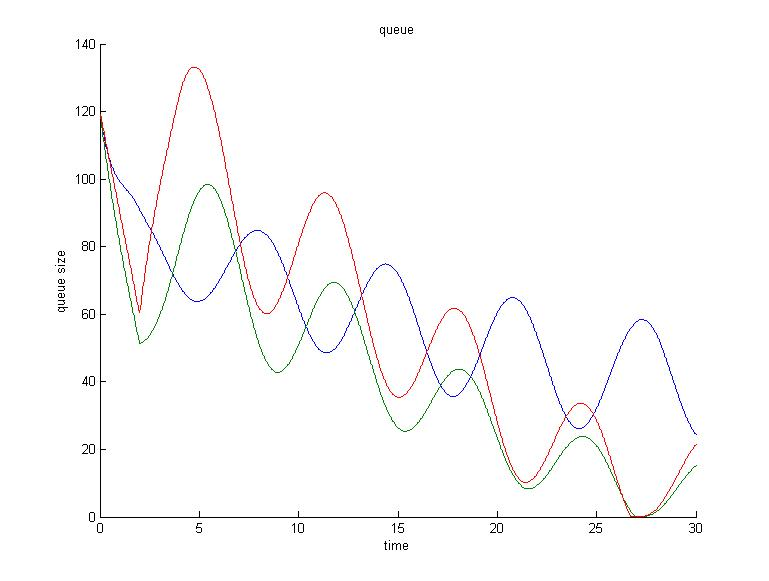
\includegraphics[width=.4\linewidth] {sinusodial_input}
\caption{Queue values vs. time with sinusoidal input instead of constant}
\end{figure}

When a sinusoidal time input is applied, the graph becomes much more energetic, with a higher rate of change and variation between graphs, a much higher rate of data transfer between the various cores, and a slightly longer computation period due to the decreased total processing power from the transfers. 

As the differential equation model includes several delayed components, the past values of the queue values is very important to the computation of the current values. for the histories, the equation:

\begin{equation} 
input=30+30\cdot sin(t\cdot4)
\end{equation}

was used to define the history of the queue size. and the resulting graph is shown below.

\begin{figure}[h]
\label{sin history}
\centering
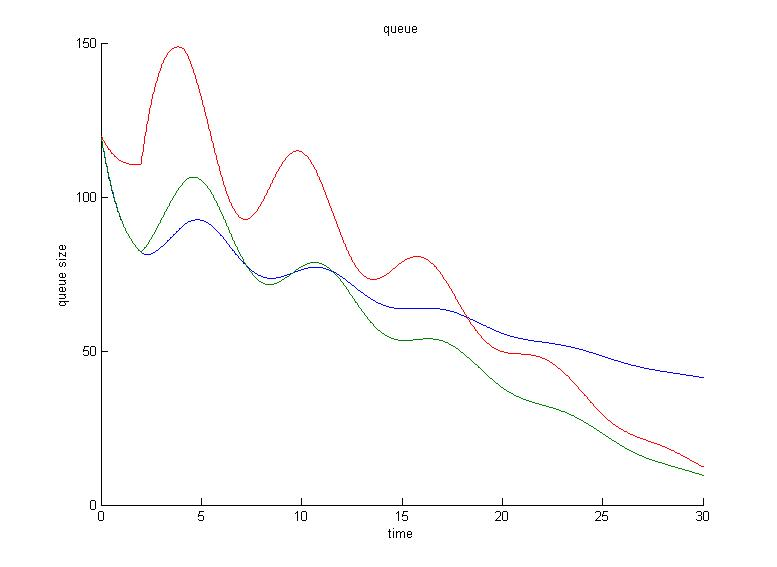
\includegraphics[width=.4\linewidth] {sinusoidal_history}
\caption{Queue values vs. time with sinusoidal history instead of constant history}
\end{figure}

When the history is made non-constant, a large effect can be seen in the first section of the graph $t<15$ seconds but this tapers off and slowly changes into a graph similar to that of the default settings, this is likely due to the effects of the damping coefficient. If the previous history was made so it was at a specific resonant frequency of the system, it is likely that the system would respond more vigorously to the sinusoidal history.

\subsection{Variations in Queue Sizes}
As discussed in section \ref{Queue Managment}, the remaining queue size above the lower limit has a significant effect on how a given core will transfer data to other cores, so the effect of changing both the lower limit floor value and the respective queue sizes is addressed. For our default model, a 1% lower bound was used on the data, such that off the bottom of the queue, 1% of the total stack size would not be transfered. To see the effects, the floor value was changed from 1% to 10% of the total value of the stack. The results on the simulation are shown below.

\begin{figure}[H]
\label{Floor increased}
\centering
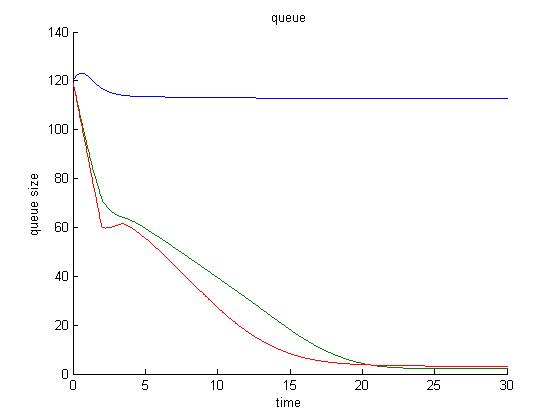
\includegraphics[width=.4\linewidth] {floor_increased}
\caption{Queue values vs. Time with an increased floor limit on the queue}
\end{figure}

As can be seen, an increase in the floor value causes the first computer to hoard all of the data in an attempt to maintain its queue, restricting both its computation and transfers.

When the queues are altered to have different queue sizes, the results of small increases in size and large increases in size can be seen below.

\begin{figure}[H]
\begin{center}
\begin{minipage}{0.45\linewidth}
\includegraphics[width=0.95\linewidth]{Queue_size_change.jpg}
\caption{Queue size vs. time for a small increase in queue size }\label{Queue small}
\end{minipage}
\begin{minipage}{0.45\linewidth}
\includegraphics[width=0.95\linewidth]{Queue_size_very_changed.jpg}
\caption{Queue size vs. time for a larger increase in queue size }\label{queue big}
\end{minipage}
\end{center}
\end{figure}

Only minimal effects can be seen from either the big or small queue changes, and mostly these changes act to decrease the flows from one computer to the next, or to deaden some of the effects of the transfers from one computer to the next. with the larger changes, these effects and an almost complete loss of the sinusoidal effects are the only effects of an increase in queue size. 


\subsection{Variations in Processing Power }
Since processing power is one of the key factors in the Load Balancing Algorithm, it was appropriate to vary the processing power in relation to the other cores. In the default system, the processing power increases by an increment of 10 between cores. Variations in the increment produced the following:
\begin{figure}[ht]
\begin{center}
\begin{minipage}{0.45\linewidth}
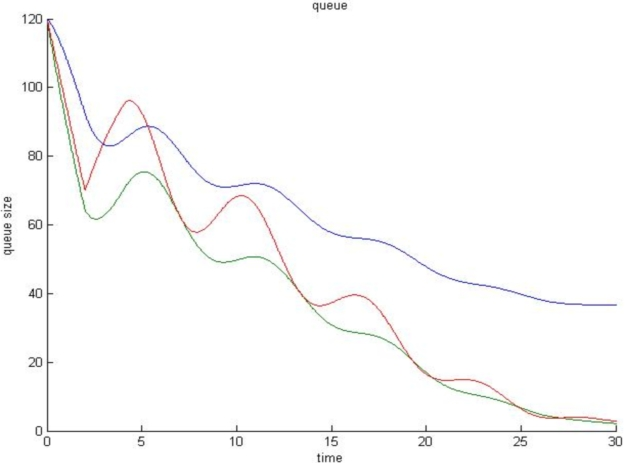
\includegraphics[width=0.95\linewidth]{./PP_less_varied.jpg}
\caption{Increment of 5}\label{LvarP}
\end{minipage}
\begin{minipage}{0.45\linewidth}
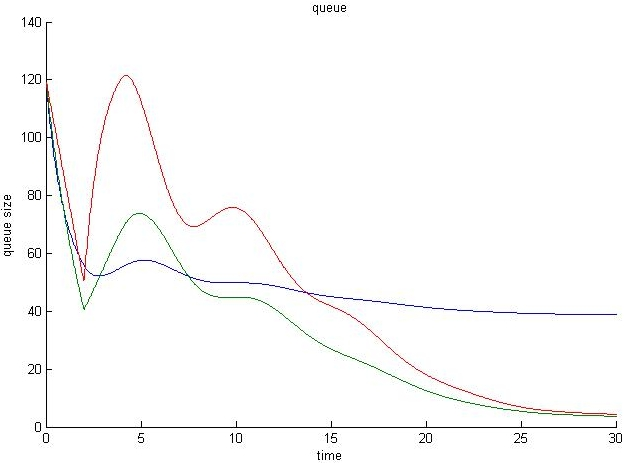
\includegraphics[width=0.95\linewidth]{./PP_more_varied.jpg}
\caption{Increment of 15}\label{HvarP}
\end{minipage}
\end{center}
\end{figure}
\\
In both of the above figures, the processing power goes from greatest to least from red to blue. In Figure \ref{LvarP} the red and the green core both receive packets from the blue core, but because their processing powers are closer together, the redistribution to the red and the green happen on a slightly different time interval, and is more gradual.In addition, the blue core holds on to the middle section of its queue much longer. In Figure \ref{HvarP} however, the green and red cores are quickly given the bulk of the blue queue at the start and the change in queue size is much more abrupt. 





\end{document}